\question 下面说法正确的是( )
\par\fourch{文件系统负责文件存储空间的管理但不能实现文件名到物理地址的转换}{在多级目录结构中对文件的访问是通过路径名和用户目录名进行的}{文件可以被划分成大小相等的若干物理块且物理块大小也可以任意指定}{\textcolor{red}{逻辑记录是对文件进行存取操作的基本单位}}
\begin{solution}图4-12为文件系统模型。可将该模型分为3个层次,最底层是对象及其属性;中间层是对对象进行操纵和管理的软件集合;最高层是文件系统提供给用户的接口。其中对对象操纵和管理的软件集合这个层次,是文件管理系统的核心部分。文件系统的功能大多是在这一层实现的,其中包括对文件存储空间的管理、对文件目录的管理、用于将文件的逻辑地址转换为物理地址的机制、对文件读和写的管理,以及对文件的共享与保护等功能,所以A是错误的。在多级目录结构中,从根目录到任何数据文件,都只有一条唯一的通路。在该路径上从树的根(即主目录)开始,把全部目录文件名与数据文件名依次用``/''连接起来,即构成该数据文件的路径名。系统中的每个文件都有唯一的路径名。所以B的说法是不准确的。对文件的访问只需要通过路径名即可。对于C选项,由于物理块大小是不可以任意指定的,它必须和外存分配方式相符合,故C错误。D正确,基于文件系统的概念,可以把数据组成分为数据项、记录和文件3级。记录是一组相关数据项的集合,用于描述一个对象在某方面的属性,是文件存取的基本单位。数据项是文件可使用的最小单位。
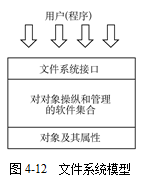
\includegraphics[width=1.48958in,height=1.89583in]{computerassets/7FB65A386B59F21177FA84BE6D2561FB.png}
\end{solution}
